\chapter{Grundlagen, Bestandsaufnahme und Vorgehen}
	\label{Kap2}
    Dieses Kapitel umfasst technische Grundlagen zu physischen Komponenten einer Energieverbundinsel mit PV-Anlage, Pufferbatterie und Ladeinfrastruktur sowie zu Standards des Energiemanagement in intelligenten Netzen. Zudem werden die Rahmenbedingungen der Hochschule für die Energieverbundinsel vorgestellt und zuletzt eine Beschreibung des methodischen Vorgehens gegeben.
%\section{Definitionen}
%	Globalstrahlung
%	diffuse Strahlung
%	Direktstrahlung


%\begin{tabular}{|c|c|c|}
%	\hline 
%	Symbol & Beschreibung & Einheit  \\ 
%	\hline 
%	 & Globalstrahlung & $\frac{kW}{m^2}$ \\ 
%	\hline 
%	 & diffuse Strahlung & $\frac{kW}{m^2}$ \\ 
%	\hline 
%	 & Direktstrahlung & $\frac{kW}{m^2}$ \\ 
%	\hline 
%	 & Test für die Autoskalierung der Tabelle ................... &  \\ 
%	\hline 
%	&  &  \\ 
%	\hline 
%\end{tabular} 

	
\section{Technische Grundlagen}
	\subsection{Photovoltaik}
		\label{Kap:PV}
		Photovoltaikmodule, auch Solarmodule genannt, sind elektrisch in Reihe geschaltete Photovoltaikzellen, auch Solarzellen genannt, und meist zusätzlich mit Rahmen und Verglasung ausgestattet. Die Zellen bestehen aus einem Halbleitermaterial und wandeln durch den Photoelektrischen Effekt kurzwellige Strahlungsenergie in elektrische Energie um. An den PV-Zellen liegt unter Bestrahlung Gleichspannung an.\\
		
		PV-Zellen werden in der Regel nach Materialart und -stärke kategorisiert. Am häufigsten sind Siliziumzellen, welche es in monokristalliner, polykristalliner, mikrokristalliner oder amorpher Ausführung gibt. Selten gibt es auch mehrschichtige Ausführungen als Tandem-Solarzelle. Abb. \ref{Abb:Vgl_PV_eta} im Anhang stellt die Entwicklung der Wirkungsgrade verschiedener Arten von PV-Zellen von 1975 bis 2017 dar.\\
		
		Die Peakleistung $P_p$, mit der Einheit $Wp$, gibt die Ausgangsleistung der PV-Anlage in $W$ bezogen auf normierte Bedingungen, den \ac{STC}, an. Die STC sind wie folgt definiert:
		\begin{itemize}
			\item Einstrahlungsstärke $G_{STC}$ von $1000 \frac{W}{m^2}$ in Modulebene
			\item Temperatur der Solarzelle $25 ^{\circ} C$ konstant
			\item Strahlungsspektrum AM 1,5 global; DIN EN 61215, IEC 1215, DIN EN 60904, IEC 904 
		\end{itemize}
		AM steht für den Begriff Air Mass, wobei die Zahl für den Faktor an Wegstrecke durch die Atmosphäre in Relation zur Atmosphärenhöhe bezeichnet. Im Winter ist dieser Wert aufgrund eines niedrigeren Einstrahlungswinkels höher. Der Weg durch die Atmosphäre verändert das Spektrum der Globalstrahlung, daher die Bezeichnung \glqq global \grqq. In Anhang \ref{Kap:PV_global} ist eine Methode zur Ermittlung des PV-Ertrags anhand der GLobalstrahlung für ebene und geneigte Flächen beschrieben.\\
		
		PV-Anlagen werden über einen Wechselrichter mit dem Wirkungsgrad $\eta_{WR}$ ans elektrische Netz angeschlossen, der den DC-Strom in 230 V, 50 Hz AC-Strom umwandelt. Mithilfe eines Smartmeters kann die Energieerzeugung gemessen und mit zeitlicher Zuordnung gespeichert werden.


		
	\subsection{Akkumulatoren}
   	\label{Kap:Akkus}
		Akkumulatoren, auch Akkus genannt, sind elektrochemische, wiederaufladbare Energiespeicher, die vor allem in mobilen Geräten als Energiequelle dienen und in der Regel aus mehreren zusammengeschalteten Akku-Zellen bestehen. Je nach Einsatzbereich wird zwischen den folgenden zwei Typen von Akkus unterschieden: \\

		\textbf{Pufferbatterien} dienen der Versorgung elektrischer Schaltungen. Sie können zum Beispiel eine \ac{USV} gewährleisten und Regelleistung bereitstellen, um fluktuierende Erzeugung und Verbrauch insbesondere bei Inselanlagen auszugleichen. \\
		
		\textbf{Traktionsbatterien} dienen dem Antrieb von Elektrofahrzeugen.
		
	\subsubsection{Speicherkapazität, State of Charge (SoC) und Ladeleistung eines Akkus}
		Bei der Speicherkapazität eines Akkus muss zwischen verschiedenen Kapazitäten differenziert werden, der theoretisch verfügbaren, brutto und netto Kapazität $W_{theo}$, $W_{brutto}$ und $W_{netto}$. Zwischen der theoretisch verfügbaren und der praktisch genutzten Kapazität gibt es, wie in Abb. \ref{Abb:kap_theo_brutto_netto} dargestellt, zwei Sicherheitsbuffer, wobei diese nicht unbedingt symetrisch vom Minimum und Maximum her angelegt sein müssen. Der erste Buffer $W_{b1}$ dient der Betriebssicherheit, damit keine zu niedrigen Zellspannungen und durch Tiefenentladung bedingte Kurzschlussbrände sowie keine zu hohen Zellspannungen, wegen Überladung auftreten. Der zweite Buffer $W_{b2}$ dient der Optimierung der Akkulebensdauer.\\
		
					\begin{figure}[h]
						\centering
						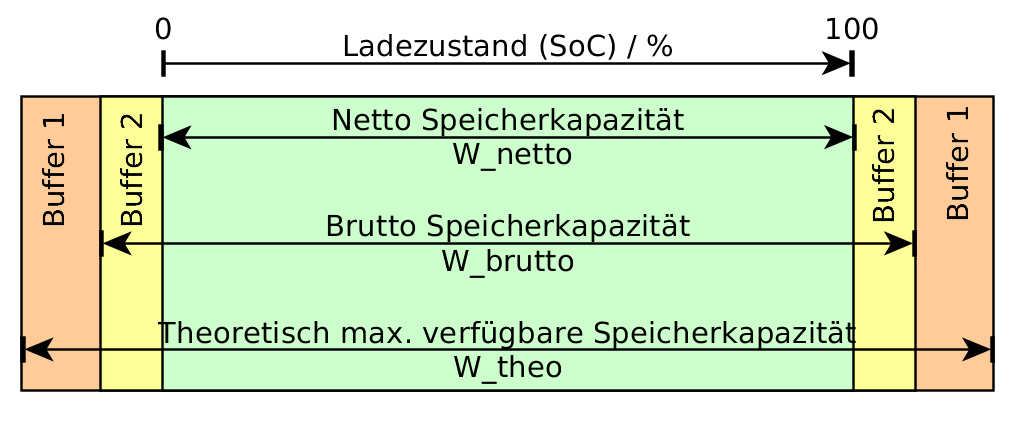
\includegraphics[width=14cm,height=5cm]{Speicherkap_theo_brutto_netto1}
						\caption{Speicherkapazitäten eines Akkus: \\
								Netto Speicherkapazität $W_{netto}$ (grün)\\
								Brutto Speicherkapazität $W_{brutto}$ (grün + gelb) \\
								Theoretisch max. verfügbare Speicherkapazität  $W_{theo}$ (grün + gelb + orange)}
						\label{Abb:kap_theo_brutto_netto}
					\end{figure}
		
		$W_{theo}$ ist die elektrochemisch, theoretisch verfügbare Kapazität eines Akkus.\\
		
		$W_{brutto}$, die brutto Speicherkapazität, ist die vom Zellhersteller freigegebene Kapazität und entspricht: $W_{brutto} = W_{theo} - W_{b1} $ \\
		
		$W_{netto}$, die netto Speicherkapazität, ist die vom Endprodukthersteller freigegebene Kapazität und entspricht: $W_{netto} = W_{brutto} - W_{b2} = W_{theo} - (W_{b1}+W_{b2})$ \\
		
		Der \ac{SoC} gibt an, wie viel Energie im Akku $W_{akku}$ bezogen auf seine netto Kapazität geladen ist: \\ $ SoC = \frac{W_{akku}}{W_{netto}}$ \\
		
		Die von einem Ladeanschluss maximal angegebene Leistung entspricht der maximalen brutto Ladeleistung $P_{brutto}$, die für den Ladevorgang maximal verbraucht werden kann. Der Akku wird dabei effektiv nur mit $P_{netto} = P_{brutto} * \eta_{charge}$ geladen, wobei $\eta_{charge}$ der Ladewirkungsgrad ist. Dieser ist das Produkt aus Wirkungsgrad des Akkus beim (Ent-)Laden und dem Wirkungsgrad des verwendeten Ladereglers. Es ist anzumerken, dass sich der Wirkungsgrad von Ladevorgängen zu dem von Entladevorgängen unterscheiden kann.\\
		
		 
%		Wichtige Kenngrößen von Akkus sind unter Anderem der \ac{SoC}, welcher den Ladezustand in Relation zum vollgeladenen Zustand angibt und der \ac{SoH}, welcher den maximal erreichbaren \ac{SoC} einer Batterie relativ zum maximal erreichbaren \ac{SoC} unter idealen Konditionen ohne Alterung angibt.  \\		
		

			
					
	\subsubsection{Batterieeigenschaften und Anforderungen}
		Akkus unterscheiden sich unter anderem durch die folgenden Merkmale von einander: Speicherkapazität, Energiedichte, Ladeleistung, Ladewirkungsgrade, ideale Temperaturbereiche für Be-/Entladung bzw. Lagerung, Zyklenfestigkeit (Lebensdauer) in Abhängigkeit der Entladetiefe (\ac{DOD}), Arbeits- und Transportsicherheit, Produktions- und Entsorgungsbedingungen, Ressourcenverfügbarkeit, mögliche Recyclinggrade, Umweltverträglichkeit sowie die Kosten für Anschaffung und Installation. \\
		
		

			
		
		\subsubsection{Batterietechnologien im Vergleich}
		%			\begin{figure}[h]
		%				\centering
		%				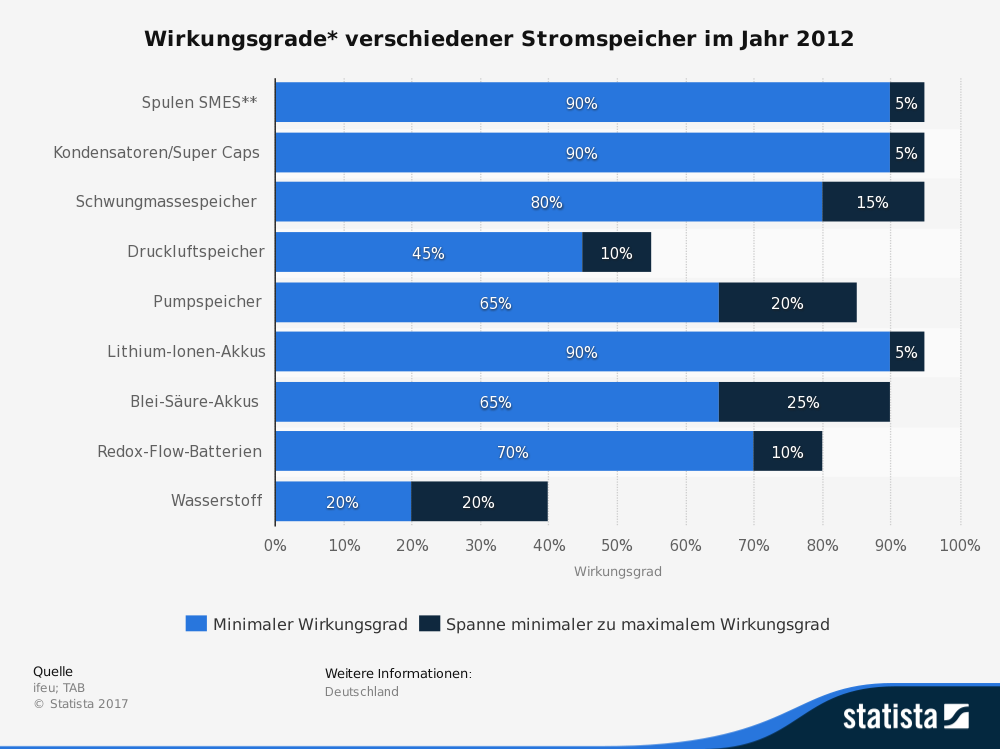
\includegraphics[width=14cm]{Batterietypen_Wirkungsgrade}
		%				\caption{Vergleich der Wirkungsgradspannbreite verschiedener Batterietechnologien im Jahr 2012 \cite[S.7]{AEE_ReNews_Strompseicher_2012} [Quelle XYZ iFEU, TAB, 2009] bzw. Renews AEE S.7}
		%				\label{Abb:Vgl_Batterien_eta}
		%			\end{figure}			
			In diesem Kapitel werden drei Speichertechnologien näher betrachtet.
			\begin{itemize}
				\item Bleisäureakkus, aufgrund dem weit verbreiteten Einsatz als Starterbatterien, Heimspeicher und für die \ac{USV}
				\item Lithiumakkus, aufgrund dem weit verbreiteten Einsatz in E-Fahrzeugen, mobilen Geräten und steigendem Gebrauch als Heimspeicher
				\item Bleikristallakkus, aufgrund der Temperaturfestigkeit, Langlebigkeit und Umweltverträglichkeit bei ähnlichem Preis wie Lithiumakkus
			\end{itemize}
			
			In Tabelle \ref{Tab:Vgl_Batterietechnologien} werden die Daten aus \cite{Comparison_Batteries_2015} zusammengefasst und um die Angaben der Wirkungsgrade und der geschätzten Kosten ergänzt. Die Kosten berücksichtigen nur die Batteriepreise ohne Ladetechnik. Zudem wurde die Zyklenfestigkeit von Bleikristallakkus, um die Herstellerangaben ergänzt, sowie die fehlenden Vorzeichen bei den Temperaturangaben in \cite{Comparison_Batteries_2015} korrigiert. Die Primärquelle ist nicht mehr verfügbar. Der angegebene Temperaturbereich entspricht mit korrigierten Vorzeichen den Entladetemperaturen anderer Quellen wie \cite{BATTUni_Temperatur}.\\ 
			
			Vertraut man den wenigen Herstellerangaben, so bieten Bleikristallakkus im stationären Einsatz als Pufferbatterie einen deutlichen Vorteil gegenüber Lithiumakkus oder herkömmlichen Bleisäureakkus. Es findet sich frappierender weise nur ein einziger Hersteller namens Betta Batteries, der seit 2009 die patentierte Lead Crystal(R) Technologie einsetzt, obwohl es bereits seit 1979 Patente für den Einsatz von Bleikristallakkus gibt. \cite{patent1}\cite{patent2} 
			
			%			Patente von 1977:
			%				http://www.freepatentsonline.com/4143216.html
			%				https://www.google.com/patents/US4140589
			
			\begin{table}[h]
				\centering
				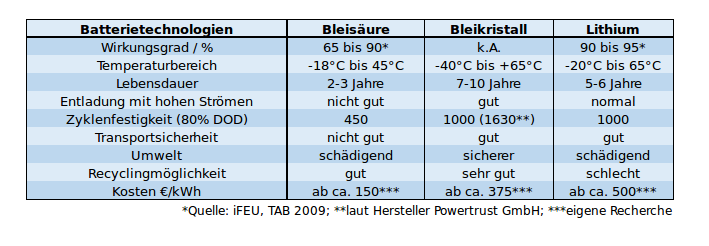
\includegraphics[width=14cm]{Vgl_Batterietechnologien}
				\caption{Vergleich von Batterien auf Basis von Bleisäure, Bleikristall und Lithium; \cite{Comparison_Batteries_2015}, *\cite[S.7]{AEE_ReNews_Strompseicher_2012}}
				\label{Tab:Vgl_Batterietechnologien}
			\end{table}

% Logisch:
%		\textbf{Sicherheitshinweis:} \\ 
%		Bei Intebetriebnahme von Pufferakkus sind ... Um die Betriebssicherheit zu gewährleisten müssen notwendige Brandschutzbedingungen beachtet werden. Je nach Akkutyp können sonst Kurzschlussbrände und Ausgasung von explosivem Wasserstoff aufgrund von Hydrolyse vorkommen. \\
	
	\subsection{Ladesysteme für E-Fahrzeuge}
		\label{Kap:Ladesysteme}
		Die internationale Norm IEC 61851 spezifiziert die elektrische Ausrüstung von Elektro-Straßenfahrzeugen u.A. konduktive Ladesysteme. 
		
		\subsubsection{E-Autos}
			\paragraph{Lademodi}
				Traktionsbatterien können sowohl mit Wechsel- als auch Gleichstrom beladen werden. In Tabelle \ref{Tab:Vgl_Ladesysteme_EAuto} werden verschiedene Lademodi für Elektro-Autos gezeigt. Die Lademodi eins bis vier für kabelgebundene Ladungen sind in der internationalen Norm IEC 62196 (in Deutschland als DIN EN 62196 gültig) zusammen mit den dazugehörigen Steckertypen spezifiziert. Für den Lademodus 5 mit kabelloser induktiver Ladung gibt es derzeit noch keine einheitliche Norm.


			\paragraph{Steckertypen}
				In Tabelle \ref{Tab:Vgl_Steckervorrichtungen} sind die üblichen Steckertypen zum Laden von E-Fahrzeugen mit Grafiken zur Bauform, Übertragungsart, mögliche Ladeleistungen und -ströme aufgelistet.
				
				\textbf{Steckertypen für AC-Ladungen} In der Norm IEC 62196-2 werden die folgenden drei verschiedene AC-Stecker normiert und mit "Typ 1" bis "Typ 3" bezeichnet. 
				
				\begin{itemize}
					\item Typ 1: SAE-J1772-2009
					\item Typ 2: Mennekes Stecker, deutscher Standard
					\item Typ 3: EV-Plug-Alliance Stecker, Erweiterung von Typ 2 mit Shuttern; findet keine Verwendung
				\end{itemize}
				
				\textbf{Steckertypen für DC-Ladungen} sind derzeit meistens eines der folgenden weltweit vorherrschenden Systeme.
				
				\begin{itemize}
					\item Combo 1, CCS (USA), basierend auf Typ 1
					\item Combo 2, CCS (Europa), basierend auf Typ 2, deutscher Standard
					\item CHAdeMO in Japan und weltweit \cite{IEC_CHAdeMO}
					\item Tesla Supercharger (exklusiv für Fahrzeuge der Marke Tesla Motors), Typ 2 modifiziert
				\end{itemize}
				
				Combo 1, Combo 2 und CHAdeMO sind durch die internationale Normen der IEC spezifiziert. \\
				
				Die beiden DC-Steckertypen \ac{CCS} Combo 1 und Combo 2 kommunizieren über Powerline Connectors und basieren wie in der Tabelle \ref{Tab:Vgl_Steckervorrichtungen} im Anhang zu erkennen auf den AC-Steckern vom Typ 1 und Typ 2. Dadurch sind Autos mit CCS-Anschluss für die AC-Stecker kompatibel. Die Kommunikation bei CHAdeMO funktioniert über einen seperaten CAN-Bus. \cite{Emobility_StatusQuo_2016} \\ 
				
				Durch die EU-Richtlinie für den Aufbau der Infrastruktur für alternative Kraftstoffe gilt europaweit Typ 2 als Standard für AC-Ladungen über 3,6 kW und Combo 2 für DC-Ladungen über 22 kW. \cite{EU_Aufbau_Infrastruktur} Mit Inkrafttreten der Ladesäulenverordnung in Deutschland wurden die Ladestecker vom Typ 2 zum Standard des AC-Ladens und die Ladestecker vom Typ Combo 2 entgegen der EU-norm auch bei DC-Ladepunkten unterhalb von 22 kW zum Standard des DC-Ladens. \cite{BMJV_LSV} \\


				
% NOTE: Interessant, aber unwichtig, da inkombatibel mit Fahrzeugen		
%			\begin{figure}[h]
%				\centering
%				\includegraphics[width=6cm]{AC_DC_Steckervorrichtung_Typ2.jpg}
%				\caption{Vergleich verschiedener Steckervorrichtungen basierend auf Typ 2 für AC- und DC-Ladung. Nur die oberste und unterste Kontaktbelegung sind normiert.}
%				\label{Abb:Vgl_Steckervorrichtungen_Typ2}
%			\end{figure}			
%			
%			[Quelle für's Bild: %http://www.mennekes.de/uploads/media/MENNEKES_Medieninformation_-_Ladesteckvorrichtungen_Typ_2_f%C3%BCr_AC_und_DC_Ladung_02.pdf 
%			]
			
			
			\paragraph{Ladeinfrastruktur für E-Autos in Deutschland}
				In Abb. \ref{Abb:BDEW_Anzahl_Ladepunkte} ist die Entwicklung der E-Mobilität in Deutschland, gemessen an der Anzahl an öffentlich zugänlichen Ladepunkten und zugelassenen Elektrofahrzeugen dargestellt.\\
					
				\begin{figure}[h]
					\centering
					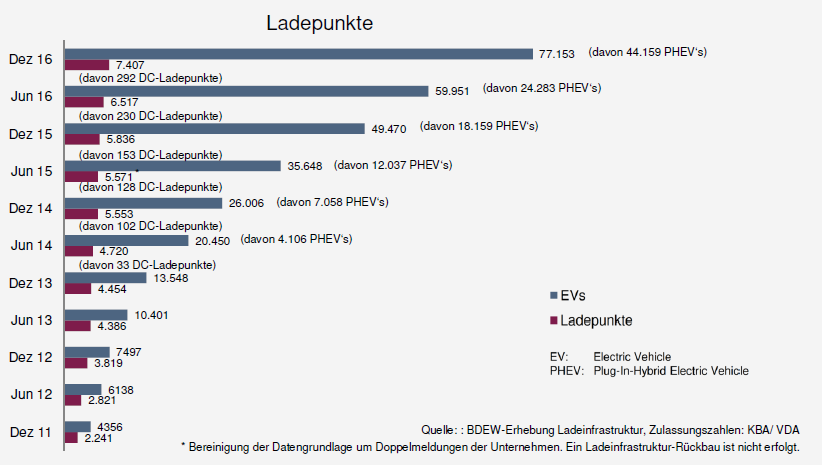
\includegraphics[width=14cm]{BDEW_Anzahl_Ladepunkte}
					\caption{Anzahl der Ladepunkte in Deutschland und EVs, Dez. 2011 bis Dez. 2016 \cite{BDEW_Anzahl_Ladepunkte}}
					\label{Abb:BDEW_Anzahl_Ladepunkte}
				\end{figure}	
			
				An den 7.407 öffentlichen Ladepunkten in Deutschland, Stand 31.12.16, sind folgende Abrechnungssysteme installiert, wobei je Ladepunkt mehrere Abrechnungssysteme möglich sind. \cite{BDEW_Anzahl_Ladepunkte} \\
				
				\begin{itemize}
					\item 4.801 RFID-Karte (rel. 65\%)
					\item 3.203 Smartphone App (rel. 43\%)
					\item 1.155 Plug'n'Charge (rel. 16\%)
					\item 1.428 Sonstige (rel. 19\%)
				\end{itemize}
			
			\subsubsection{E-Motorräder und E-Roller}
				E-Motorräder können mit dem entsprechenden Ladezubehör an jeder herkömmlichen Schuko-Steckdose geladen werden. Eine öffentliche Ladeinfrastruktur mit Schnelladepunkten ist derzeit noch nicht verfügbar.
				
				Hersteller für Elektro-Motorräder und Zubehör wie Zero Motorcycles bieten auch externe Schnelladegeräte wie den Charge Tank mit 6 kW Ladeleistung als Ergänzung zum internen Ladegerät mit ca. 1,5 kW ihrer Fahrzeuge an. Dieser kann an Level-2-Ladestationen, mit Steckertyp 2, angeschlossen werden.[Quelle] 
			
%			Beispielfahrzeuge:
%			QvR VR One 
%				https://www.adac.de/_mmm/pdf/ADAC%20Fahrberichte%20_%20QvR_91kb_122015.pdf
%			Vectrix VX-1 LI+ 
%				https://www.adac.de/_mmm/pdf/ADAC%20Fahrberichte%20_%20ZeroVectrix_92kb_122013.pdf
%			ZERO DS 
%				https://www.adac.de/_mmm/pdf/ADAC%20Fahrberichte%20_%20Zero_91kb_122014.pdf
			
			
			\subsubsection{E-Bikes und Pedelecs}
				Fast alle Elektrofahrräder können mit Ladekabel und Netzteil an einer herkömmlichen 230 V Schuko-Steckdose geladen werden.\\
				
				Die häufigsten Formen von Fahrradladestationen sind:
				\begin{itemize}
					\item Fahrradständer mit angebrachten Steckdosen
					\item Abschließbare Akkuschränke mit im Innern angebrachten Steckdosen
					\item Ladesäule mit angebrachten Steckdosen 
					\item Ladesäule mit eigenem Kabelsystem (z.B. von bike-energy)
				\end{itemize}
				
				% Bike energy 
				% http://www.bike-energy.com/


		\subsection{Energiemanagement im intelligenten Stromnetz}
		\label{Kap:Grundlagen_Energiemanagement}
		% Einleitung
		In diesem Kapitel wird das Konzept und das Ziel von Energiemanagement beschrieben und es werden verschiedene Standards für Smart Grid Anwendungen vorgestellt. 	
		
		\subsubsection{Definition Energiemanagement, Energymanagementsystem (EMS), Smartgrid}
		% Definition Energiemanagement
			\glqq Energiemanagement ist die Kombination aller Maßnahmen, die bei einer geforderten Leistung einen minimalen Energieeinsatz sicherstellen. Es bezieht sich auf Strukturen, Prozesse und Systeme sowie auf menschliche Verhaltensweisen und -änderungen.\grqq \cite{Def_Energiemanagement} Damit umfasst Energiemanagement die Planung und den Betrieb energietechnischer Verbrauchs- und Erzeugungseinheiten, im folgenden \ac{CPS}-units genannt. \\ 
			
		% Definition Energiemanagementsystem
			Ein \ac{EMS} dient der systematischen Erfassung, Kommunikation und Regelung von Energieflüssen z.B. durch Smart Metering und der automatisch auf einander abgestimmten Steuerung mehrerer Geräte.\\
			
		% Definition Smart Grid
			Ein intelligentes Stromnetz (englisch Smart Grid) ist eine Form eines \ac{EMS}. Ein Smart Grid umfasst die kommunikative Vernetzung und Steuerung von CPS-units, wobei abhängig von den Ausmaßen des Smart Grids auch von Microgrids und Nanogrids gesprochen wird. Eine normierte Definition der Bezeichnungen gibt es (noch) nicht. \\
			
		\subsubsection{Ziele von und Ansätze für Energiemanagement}
		% Ziele
			Die Energieflüsse können hinsichtlich verschiedener Gesichtspunkte optimiert werden. Ziele können u.A. sein:
			\begin{itemize}
				\item Energiekostensenkung
				\item Ressourcenschonung
				\item Verbesserung der Netzstabilität und Versorgungssicherheit
				\item Autarkiegraderhöhung durch bessere Nutzung eigenproduzierter Energie
			\end{itemize}

		% Ansätze
			Smart Grids können abhängig von der Architektur u.A. die folgenden Möglichkeiten für Energiemanagement bereit stellen:
			\begin{itemize}
				\item Smart Metering (Erfassung und Kommunikation von Messdaten durch intelligente Zähler)
				\item Bereitstellung von Regelleistung (durch Regelung oder Abschaltung von CPS-unit wie sz.B. Pumpspeicherkraftwerke, konventionelle Dampfkraftwerke, BHKWs, Biogas- und Müllverbrennungsanlagen, Batteriespeicher, Lüftungs- und Kühlsystemen, elektrischen Heizsystemen)
				\item Automatisches \ac{DSM} durch Einsatz von \ac{GFA} Controllern zur Primärregelung der Netzfrequenz ohne zentrale Steuerung und ohne Kommunikation mit anderen CPS-units
			\end{itemize}

% GFA Quelle:
%				http://ieeexplore.ieee.org/document/6732970/?reload=true&tp=&arnumber=6732970&refinements%3D4291944246%26ranges%3D2014_2015_p_Publication_Year%26queryText%3DFPGA
% https://www.researchgate.net/publication/224188933_Frequency_waves_Grid_Friendly_Appliances_and_geographic_limits_in_a_smart_grid



			% Schema mit Hardwarekomponenten, verschiedenen Bussystemen und Steuereinheit
			
			\subsection{Smart Grid Architecture Model (SGAM) Framework}
				Das \ac{CENELEC} hat einen Bericht der Smart Grid Coordination Group und Reference Architecture
				Working Group veröffentlicht mit der Beschreibung des \ac{SGAM} Framework, einem interoperablen Modell für Smart Grid Architekturen. Ziel des SGAM ist es, aus verschiedensten Standards ein umfängliches, kompatibles, konzeptuelles Modell mit holistischem Ansatz als für alle Anwendungsfälle unabhängig von der angewandten Technologie zu erstellen. \cite{CENELEC_SmartGrid} \\
                
				Einige solcher sich teilweise überschneidender Standards sind beispielsweise die "German standardization roadmap E-Energy" des \ac{DKE}, die IEEE Standards IEEE SCC21 (Standards Coordinating Comittee on Fuel Cells, Photovoltaics, Dispersed Genreration, and Energy Storage), P2030 (Standard Interoperability Smart Grid Concepts) und die Framework und Roadmap for Smart Grid Interoperability Standards, das \ac{NIST EA Model}. \cite{DKE_SmartHome} \\ %NOTE: cite XYZ IEEE standards
				
				%NOTE: Warum werden einige dem SGAM zugrunde liegenden Standards aufgelistet?
				
				Der Aufbau des SGAM Frameworks wird ausführlich in Anhang \ref{Kap:SGAM_aufbau} beschrieben.
				
		

			\subsubsection{Open Gateway Energy MAnagement 2.0 (OGEMA 2.0)}
				\ac{OGEMA} 2.0 ist ein open source Software-Framework und dient als Programmierschnittstelle für Energiemanagement Anwendungen. Es ermöglicht die Realisierung von Energiemanagementsystemen für Gebäude, den industriellen Bereich und die Elektromobilität. Das Framework nutzt, wie in Abb. \ref{Abb:OGEMA_Aufbau} zu sehen ist, eine Java-Plattform und standardisierte Datenmodelle für verschiedenste Energieerzeuger, -verbraucher und -speicher. Die Software ist hardwareunabhängig und kann somit leicht an andere Plattformen adaptiert werden. \cite{OGEMA_Praes} \\
                
				Entwickelt wurde OGEMA mit Förderungen des Bundesministeriums für Wirtschaft und Energie von den drei Fraunhofer Instituten für Windenergie und Energiesystemtechnik (IWES), für integrierte Schaltungen (IIS) und für solare Energiesysteme (ISE). Derzeit gibt es verschiedene Projekte in denen Smart Grid Anwendungen mit OGEMA getestet werden, darunter eines in Mannheim. \cite{ogemamoma}
				
				\begin{figure}[h]
					\centering
					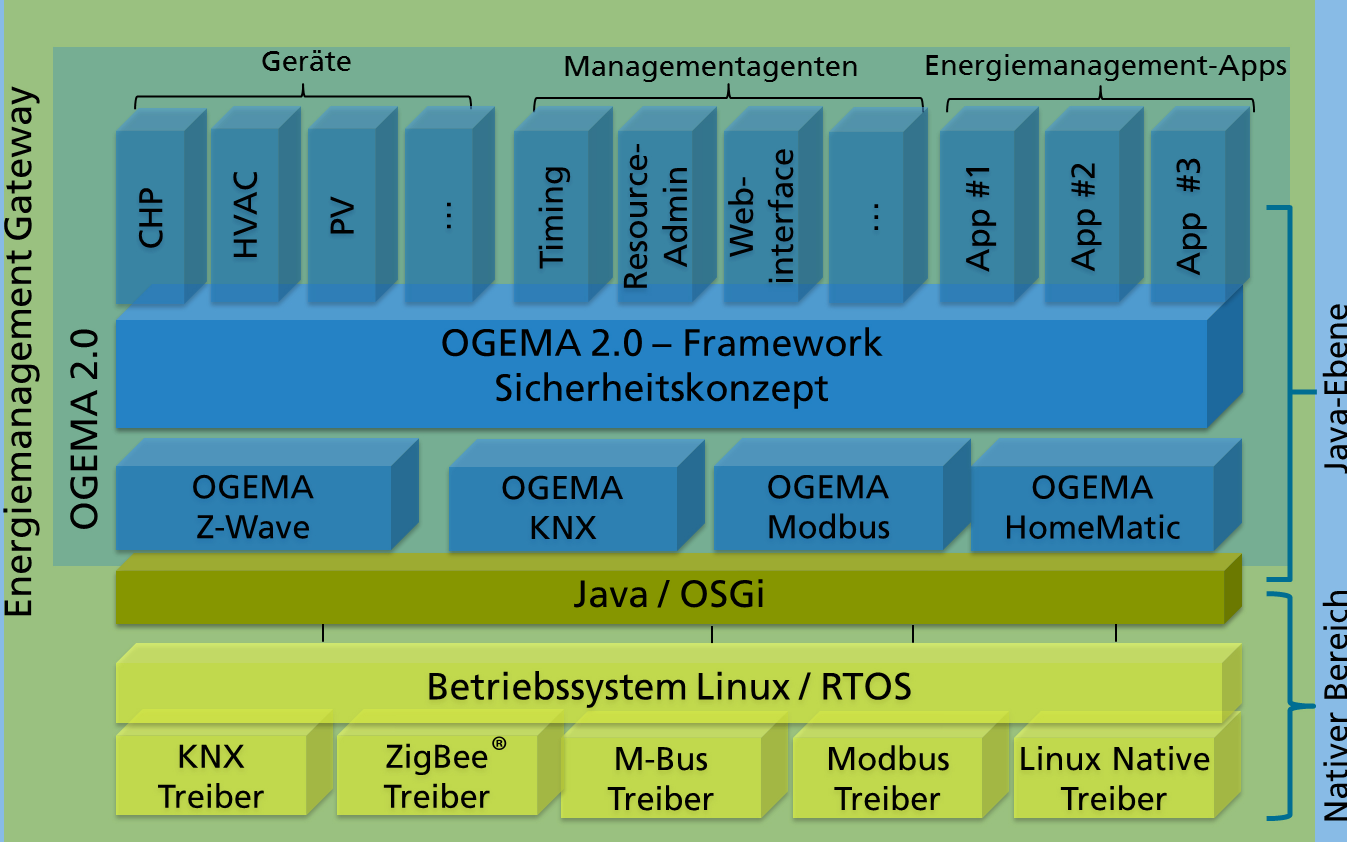
\includegraphics[width=14cm]{OGEMA}
					\caption{Modulare Baukastenstruktur von OGEMA \cite{OGEMA_Praes}}
					\label{Abb:OGEMA_Aufbau}
				\end{figure}			
	
%				Im Zuge dieser Bachelorarbeit war es nicht möglich das OGEMA 2.0 Demokit auf den Betriebssystemen Windows 7, Windows 10 und XUbuntu (s. Abb. \ref{Abb:OS_java_ubuntu}) zu starten.\\
				
%				Version des Betriebssystems und Javas unter XUbuntu: \\
%				Distributor ID:	Ubuntu \\
%				Description:	Ubuntu 16.04.4 LTS \\
%				Release:	16.04 \\
%				Codename:	xenial \\
%				openjdk version "1.8.0\_162" \\
%				OpenJDK Runtime Environment (build 1.8.0\_162-8u162-b12-0ubuntu0.16.04.2-b12)\\
%				OpenJDK 64-Bit Server VM (build 25.162-b12, mixed mode)\\
				
				
%				\begin{figure}[h]
%					\centering
%					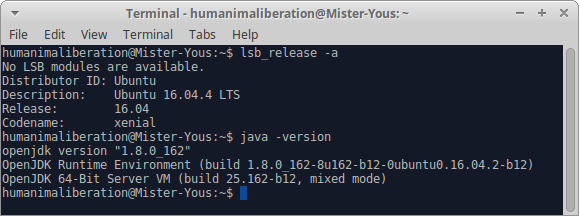
\includegraphics[width=14cm]{OS_java_ubuntu}
%					\caption{Version von Betriebssystem und Java der laufenden XUbuntu Distribution}
%					\label{Abb:OS_java_ubuntu}
%				\end{figure}			
				
				%NOTE XYZ Win 10 
				
%				https://www.energy-seeds.org/content/dam/energy-seeds/de/documents/22_2014-10-27_Energiesymposium_FhG-IIS-Heusinger_Flexible-Softwarplatforem-Energiemanagement.pdf



				
			\subsubsection{EEBUS und Smart Premises Interoperable Neutral-message Exchange (SPINE)}
				Das EEBUS Datenmodell ist Bestandteil internationaler Standards:
				
				\begin{itemize}
					\item CENELEC EN 50631 (Interoperable Connected Household Appliances) \cite{CENELEC}
					\item ETSI TS 103 410-1 SAREF4ENER (EU Framework SAREF; Smart Appliances REFerence) \cite{Etsi}
				\end{itemize}
							EEBUS ist trotz des Namens kein Bus-System, sondern ein offener Standard für eine Kommunikationsschnittstelle, die von jedem Gerät und jeder technischen Plattform unabhängig von Hersteller und Technologie genutzt werden kann. Somit ermöglicht EEBUS energietechnisch relevanten Geräten im \ac{IoT} in einer standardisierten Sprache für Steuerung und Management miteinander zu kommunizieren. \\ %Ev. auch wichtig ISA‐62443‐1‐4SecurityLifecycleundUseCases–auchbekanntalsISA 99


			
				
				Die zugrundeliegende Technik von EEBUS ist die Datenmodell-Spezifikation von \ac{SPINE} wie in Abb. \ref{Abb:EEBUS_Spec} im Anhang dargestellt. \\
				
				Entwickelt wird der EEBUS-Standard von dem 2012 gegründeten gemeinnützigen Verein EEBus Iniative e.V., der von Vertretern namenhafter Unternehmen aus der Industrie als auch des europäischen Komitees für elektrotechnische Normung CENELEC geleitet wird. Hervorgegangen ist EEBUS aus dem Projekt Smart Watts des Förderprogramms E-Energy, das vom Bundesministerium für Wirtschaft und Technologie (BMWi) und dem Bundesministerium für Umwelt, Naturschutz und Reaktorsicherheit (BMU) aufgelegt wurde.\\

				\paragraph{SPINE}
				\ac{SPINE} definiert Nachrichten und Verfahrensweisen nur auf der Anwendungsebene nach dem ISO-standardisierten \ac{OSI-Modell}. Das OSI-Modell beschreibt 7 Ebenen für die Kommunikation zwischen zwei Systemen, von der Anwendungsebene über die (optionale) Darstellungs- und (optionale) Sitzungsebene, über die Transport-, Vermittlungs- und Sicherungsebene zur Bitübertragungsebene. Abb. \ref{Abb:EEBUS_Spec} zeigt die Abgrenzung zur Transportebene. Es ist damit komplett unabhängig vom gewählten Transportprotokoll. In Abb. \ref{Abb:SPINE_SGAM_Layers} ist SPINE im \ac{HBAM}, eingeordnet, welches sich vom \ac{SGAM} ableitet. \\
				
				\begin{figure}[h]
					\centering
					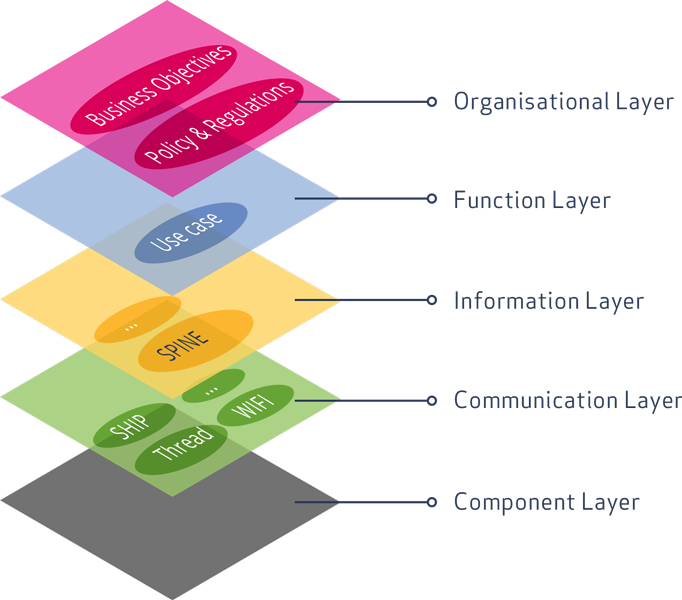
\includegraphics[width=8cm]{SPINE_SGAM_Layers}
					\caption{Einordnung von SPINE in das \ac{SGAM} sowie der daraus abgeleiteten \ac{HBAM} \cite{EEBUS_Web}}
					\label{Abb:SPINE_SGAM_Layers}
				\end{figure}			
				
				Die nach SPINE-Spezifikation normierten Datenmodelle sind interoperable und für verschiedene Protokolle und Übertragungswege nutzbar. Damit ist es beispielsweise mit WLAN oder KNX, welches in der Gebäudetechnik weit verbreitet ist, kompatibel. Mit entsprechenden Treibern müsste das SPINE-Datenmodell auch mit OGEMA-Anwendungen kompatibel sein.\\
				
				Das SPINE-Datenmodell umfasst Datensätze für Anwendungsfälle (use cases) mit Metadaten z.B. über die jeweiligen physikalischen und logischen Gerätetypen (device and entity type) und Funktionalitäten (features) sowie komplexe Klassen und Standard-Klassen mit konkreten Funktionen für die Steuerung der jeweiligen Geräte. \cite{EEBUS_Intro} \\

			\subsubsection{Open Charge Point Protocol (OCPP)}
				Das Protokoll OCPP definiert die Kommunikation zwischen Ladepunkt und Zentralsysten, nicht aber die verwendete Kommunikationstechnologie. Jede Technologie, die TCP/IP-Verbindungen unterstützt kann eingesetzt werden. Die verschiedenen Versionen sind aufgrund neuer Eigenschaften nicht unbedingt rückwirkend kompatibel. Im März 2018 kam die derzeit aktuelle Version 2.0 heraus. In der Version 1.5 und 1.6 gab es noch erhebliche Sicherheitsprobleme, die neben anderen in Kapitel \ref{Kap3} erwähnt werden. \cite{CCC} \cite{evsim} 
	
						
				
		\subsection{Autarkiegrad und Eigenverbrauchsanteil}
			Der Autarkiegrad eines Systems kann hinreichendes Bewertungskriterium zur Optimierung dessen Energieflüssen sein. Er gibt den relativen Anteil der verbrauchten Energiemenge im System an, die innerhalb des Systems erzeugt werden kann. Ein Autarkiegrad von 100\% bedeutet demnach ein energieautarkes System, welches die Menge an benötigter Energie selbst erzeugen kann.\\
			
			$Autarkiegrad = \frac{Erzeugte\, Energie\, im\, System}{Verbrauchte \,Energie\, im\, System}$ \\
			
			Der Eigenverbrauchsanteil hingegen gibt den relativen Anteil der von einem System erzeugten Energiemenge an, die darin selbst verbraucht wird. Ein Eigenverbrauchsanteil von 100\% bedeutet nur, dass die gesamte erzeugte Energie des Systems von diesem selbst verbraucht wird. \\
			
			$Eigenverbrauchsanteil = \frac{Erzeugte\, Energie\, im\, System,\, die\, im\, System\, verbraucht\, wird}{Erzeugte\, Energie\, im\, System}$
			
			

						
\section{Rahmenbedingungen}
	\label{Kap:Rahmenbedingungen}
	\subsection{Standortanalyse}
	Abbildung \ref{Abb:Campusplan} zeigt den Campusplan der Hochschule Mannheim. Der Standort vor dem Hochspannungslabor, Gebäude F, für zwei Container der Energieverbundinsel wie in der Planung von Frau Ong vorgesehen, wurde von der Stadt abgelehnt. \cite{BA_Chris_Ong_2017} Die Ladesäule vor der Bibliothek, Gebäude L, wurde abgebaut und dafür wurde zwischen Gebäude B und Grünfläche eine Ladesäule mit einem einzelnen Stecker des Typ 2 und einer maximalen ladeleistung von 22 kW errichtet. Ein weiterer Ausbau der Ladeinfrastruktur ist gegenwärtig (im Mai 2018) noch nicht geplant.
    
		\begin{figure}[h]
			\centering
			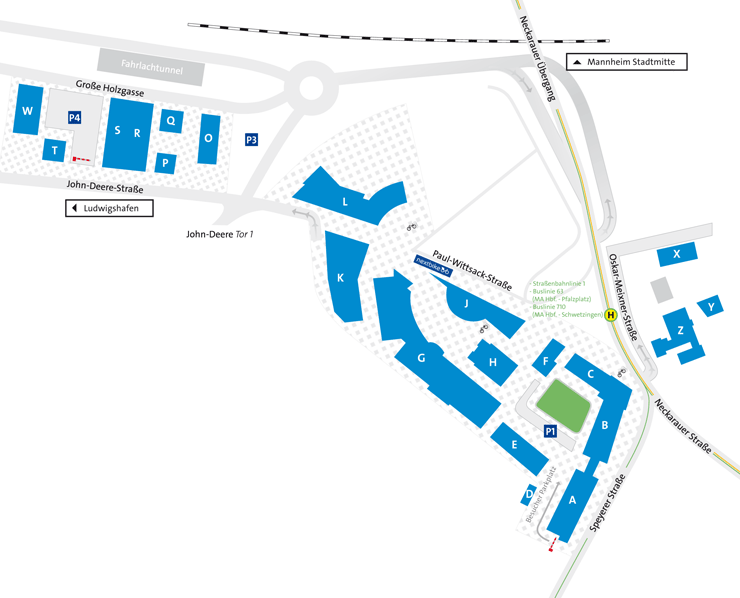
\includegraphics[width=0.9\textwidth]{campusplan_edit}
			\caption{Campusplan der Hochschule Mannheim \cite{HS_Campusplan}}
			\label{Abb:Campusplan}
		\end{figure}			

	\subsection{E-Fahrzeuge}
		\label{Kap:Fahrzeuge}
		Die Hochschule Mannheim besitzt zwecks Forschung und Fortbewegung für Mitarbeiter*innen eine Reihe verschiedener E-Fahrzeuge. Diese sind in Tabelle \ref{Tab:EFahrzeuge_Liste} mit einer Typenbezeichnung, der Batteriekapazität und den verfügbaren Ladeoptionen aufgelistet. Die Fahrzeugflotte der Hochschule Mannheim ist nicht repräsentativ für die E-Fahrzeuge im deutschen Straßenverkehr, werden vorraussichtlich aber den Großteil der zu ladenden Vehikel in der Energieverbundinsel darstellen.  \\
		
		Neben den Hochschulfahrzeugen werden zusätzlich der Zoe Z.E.40 von Renault, der i3 von BMW und der fortwo von Smart mit optionalem 22kW-Bordlader als Referenzautos angegeben. Der Zoe ist in Deutschland das E-Auto mit den meisten Neuzulassungen 2017. Der i3 liegt auf Platz 2 und war  im Vorjahr auf Platz 1 der Neuzulassungen. Gegenüber dem Stromos besitzen beide Fahrzeuge eine höhere Batteriekapazität und mögliche Ladeleistung. \cite{EAutos_Ranking}
		
		\begin{table}[h]
			\centering
			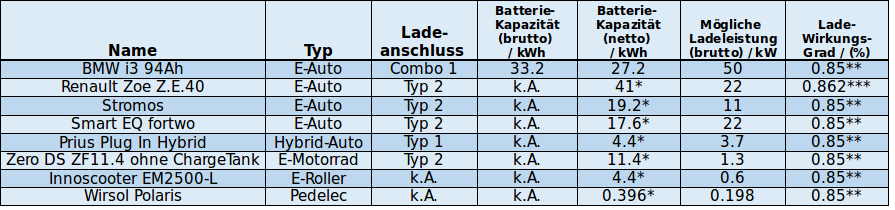
\includegraphics[width=14cm]{EFahrzeuge_Liste}
			\caption{Liste verschiedener E-Fahrzeuge mit Kenndaten nach Herstellerangaben\cite{spec_i3} \cite{spec_i3eng} \cite{spec_zoe} \cite{spec_stromos} \cite{spec_smart} \cite{spec_prius} \cite{spec_zero} \\ *Annahme: Herstellerangabe ist brutto Kapazität mit 85\% netto Kapazität
			\\ **eigene Schätzung
			\\ ***Mittelwert von Messungen eines Fahrzeugnutzenden \cite{spec_zoeeta}}
			\label{Tab:EFahrzeuge_Liste}
		\end{table}			
		
    \subsection{Kenndaten der PV-Anlage}
		In Tabelle \ref{Tab:PV_kenndaten} sind die Kenndaten der PV-Anlage und des PV-Wechselrichters (PV-WR) auf Gebäude C der Hochschule Mannheim aufgelistet. Die Kenndaten sind den Herstellerspezifikationen im Anhang \ref{Kap:datasheet_pv_wr} entnommen. 
		
		\begin{table}[h]
			\begin{tabular}{|c|c|c|}
				\hline 
				 							& \textbf{Wert / Modellbezeichnung} & \textbf{Einheit} \\ 
				\hline 
				PV-Module 							& REC PE 265 Wp &   \\ 
				\hline 
				Peakleistung PV-Modul unter STC 	& 265 		& Wp \\ 
				\hline
				Wirkungsgrad PV-Modul unter STC 	& 16,1 		& \%  \\ 
				\hline 
				Modulfläche 						& 1,65 		& $m^2$  \\ 
				\hline 
				Anzahl PV-Module 					& 76 		& \\ 
				\hline  
				Peakleistung PV-Anlage unter STC	& 20,145 	& kWp  \\ 
				\hline 
				PV-Wechselrichter (PV-WR) 			& SAM STP 20.000 TL-þ30 & \\ 
				\hline
				Wirkleistung PV-WR 					& 14,09 	& kW\\
                									& (reduziert auf 70\%)   &\\ 
				\hline
				PV-WR: NA-Schutz 					& integriert &\\ 
				\hline
			\end{tabular} 
			\caption{Kenndaten der PV-Anlage auf Gebäude C der Hochschule Mannheim} %NOTE XYZ REF Anhang Datenblatt
			\label{Tab:PV_kenndaten}
		\end{table}
		
		
% NOTE: Fehlt noch:
%		Keine Verschattung
%		Modulausrichtung:
%		Modulneigung: Hälfte 7,72°, andere Hälfte -7,72°

		


		
	\subsection{Vorgaben bei der Dimensionierung}
		\label{Kap:Vorgaben}
		
		% Grundkonzept und Pmax der gesamten Ladeinfrastruktur
		Die Energieverbundinsel soll Lademöglichkeiten für 3 Autos, 2 Motorräder und 5 Fahrräder besitzen. Der Anschluss ans Hochschulnetz ist dabei auf eine verfügbare Leistung $P_{max}$ von maximal 50 kW + 20 \% Reserve begrenzt. Abbildung \ref{Abb:Netztopologie} zeigt den schematischen Aufbau der relevanten CPS-units in der Energieverbundinsel.\\

		Die Dimensionierung der Ladepunkte erfolgt unter Berücksichtigung von $P_{max}$ und den üblicherweise für E-Fahrzeugen ausgelegten Ladeleistungen (s. Kapitel \ref{Kap:Fahrzeuge}) mit den in Tabelle \ref{Tab:Ladepunkte} aufgelisteten Steckertypen und Anschlussleistungen. \\
        
		\begin{figure}[h] % Netztopologie
			\centering
			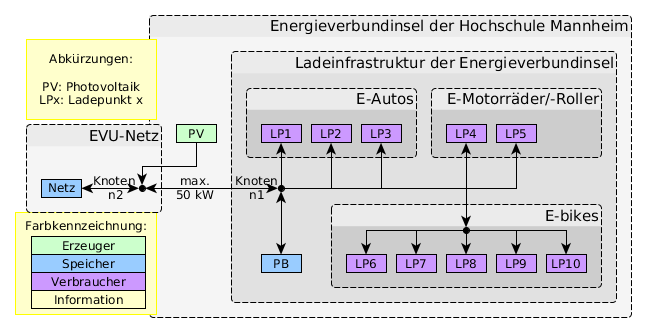
\includegraphics[width=14cm]{Netztopologie1}
			\caption{Geplante Netztopologie der Energieverbundinsel}
			\label{Abb:Netztopologie}
		\end{figure}		
			
		\begin{table}[h]
			\centering
			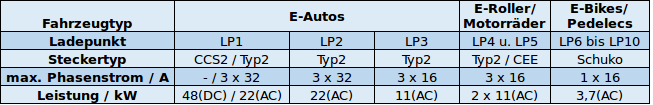
\includegraphics[width=14cm]{Ladepunkte}
			\caption{Übersicht der Ladepunkte nach Fahrzeug- und Steckertyp, Anzahl der Phasen, maximalem Phasenstrom und maximaler Ladeleistung}
			\label{Tab:Ladepunkte}
		\end{table}	
	
		Die Summe der maximalen Ladeleistung aller Ladepunkte einzeln liegt bei 106,7 kW und übersteigt die Übertragungskapazität von 50 kW am Anschluss der Ladeinfrastruktur ans Hochschulnetz. Die Anforderungen an ein EMS zur Steuerung von Ladepunkten und einer Pufferbatterie zur Einhaltung der Grenzwerte der Übertragungsleistung am Anschlusspunkt wird in Kapitel \ref{Kap3} beschrieben.\\
		
		Für eine vollständige Kompatibilität mit allen in Kapitel \ref{Kap:Ladesysteme} vorgestellten Ladesystemen können Adapter von Typ 2 auf Typ 1 sowie Adapter von CCS2 auf CCS1 zur Verfügung gestellt werden.\\
		
%	\subsection{Rechtlich}	
%		Ggfs. diese subsection löschen	

%		- Eigentumsrecht \\
%		- Parkplatz \\
%		- Baugenehmigung erforderlich? Vorraussetzungen? \\
%		- - Fundamentbau \\
%		- - Mobiler Container \\
%		- PV Anlage, Direkteinspeisung ins Microgrid \\
%		- Batterienutzung, Normen, Sicherheit\\
%		- Registrierung Ladestelle? \\

	
				

\section{Methodisches Vorgehen für die Energieflussberechnung}
% Kap3 (Anforderungen EMS)
	% Konzept: Use-Case, SGAM Mapping
	% Unvollständiges SGAM Mapping: Function Layer, Component Layer, Information Layer 
	% Ausstehend im SGAM Mapping: Communication Layer, Business Layer
	Aufbauend auf den vorgegebenen Rahmenbedingungen aus Kapitel \ref{Kap:Vorgaben} wird in Kapitel \ref{Kap3} der Use Case eines Nanogrids mit konfigurierbarer, teilautarker Ladeinfrastruktur definiert. Für die Energieverbundinsel wird ein EMS mit einstellbaren Ladesequenzen konzipiert. Die Anforderungen an einzelne Teilbereiche im SGAM werden erläutert insoweit sie für die Simulation der Energieflussberechnung notwendig sind. Die Teilbereiche, welche darüber hinaus für die praktische Implementation, nicht jedoch für die Simulation nötig sind, werden nur angedeutet.\\

% Kap4 (Einergieflussberechnung)
	% Randbedingungen, Szenarienfestlegung
	% Code beschreiben
	% Simulationsergebnisse
	% Simulationsauswertung	
	Die einzelnen Szenarien werden in Kapitel \ref{Kap4} mit entsprechenden Randbedingungen für die Energieflussberechnung definiert und simuliert. Für die Erstellung von Erzeugungsprofilen der PV-Anlage wird ein Matlab-Code programmiert, um Wetterdaten des DWD auszuwerten und anhand der Globalstrahlungsdaten und Kenndaten der PV-Anlage die Leistung zu ermitteln. Für die Simulation der Energieflüsse wird ein weiterer Matlab-Code entworfen, der auf den zuvor in Kapitel \ref{Kap3} bestimmten Anforderungen an ein EMS aufbaut. Die Programme werden so entworfen, dass sich durch Variation der Parameter leicht weitere Szenarien untersuchen lassen. \\

% Kap5 
	% Ergebniszusammenfassung
	% Handlungsempfehlung
	% Ausblick
% Kap6 (Fazit)
	In Kapitel \ref{Kap5} werden die Simulationsergebnisse zusammengefasst und ausgewertet. Aus den Ergebnissen werden Handlungsempfehlungne für die Dimensionierung und die Betriebsweise der Energieverbundinsel abgeleitet. Dazu wird ein Ausblick gegeben, der Möglichkeiten zur Weiterentwicklung des Konzeptes Energieverbundinsel präsentiert. Zum Schluss werden Auswertung, Handlungsempfehlung und Ausblick in einem Fazit in Kapitel \ref{Kap6} zusammengefasst.

	\subsection{Verwendete Software}
		Für diese Studie wurde vorzugsweise frei verfügbare Open Source Software verwendet, welche im folgenden gelistet ist.
	
		\subsubsection{Projektplanung: GanttProject}
			GanttProject ist eine freie Anwendung für Projektplanung, mit der Gantt-Diagramme wie in Abb. \ref{Abb:gantt} erstellt werden können. Dies erleichtert durch die übersichtliche Visualisierung in von zeitlich zugeordneten Blöcken von Projektphasen die Zeitplanung von zeitlich voneinander abhängigen Arbeitsschritten. \cite{gantt}
		
		\subsubsection{Dokumentation: LaTeX}
			Dieser Bericht wird mithilfe der LaTeX-Vorlage für Abschlussarbeiten an der Hochschule Mannheim geschrieben. \cite{latex_template} LaTeX ist ein quelloffenes, frei verfügbares Softwarepaket, das die Benutzung des Textsatzsystems TeX durch Makros vereinfacht. Das LaTeX-Format erfordert eine bestimmte Syntax aufgrund der code-basierten Schreibart, was zu einer höheren Einarbeitungszeit als bei den verbreiteten Texteditoren wie Word, Open Office und Libre Office führt. LaTeX bietet demgegenüber zahlreiche Vorteile unter Anderem beim Darstellen mathematischer Formeln, Referenzieren und Zitieren, was wichtige Bestandteile wissenschaftlicher Dokumentationen sind. \\
			
		\subsubsection{Programmablaufpläne: yEd Graph Editor}
			Der Diagrammeditor yEd ist eine proprietäre, kostenlos nutzbare, plattformunabhängige Software zur Erstellung verschiedenster Diagrammtypen wie beispielsweise Programmablaufpläne und wurde für die im Kontext dieser Arbeit entstandenen Blockdiagramme und Programmablaufpläne verwendet. \cite{yed}
			
		\subsubsection{Programmiersprache: Matlab, Integrierte Entwicklungsumgebung: Gnu Octave}
			Die Simulationsprogramme werden unter Verwendung von Gnu Octave in Matlab-Code (.m-Code) geschrieben. Matlab ist eine häufig verwendete proprietäre Software im wissenschaftlich-technischen Bereich zur Lösung mathematischer Probleme und graphischen Darstellung, vor allem ausgelegt auf die numerische Berechnung mithilfe von Matrizen. Gnu Octave ist ein Open Source Klon Matlabs mit Fokus auf Kompatibilität zu Matlab generierten .m-Code mit überwiegend identischer Syntax. \\
	